\documentclass[sigconf]{acmart}
% defining the \BibTeX command - from Oren Patashnik's original BibTeX documentation.
\def\BibTeX{{\rm B\kern-.05em{\sc i\kern-.025em b}\kern-.08emT\kern-.1667em\lower.7ex\hbox{E}\kern-.125emX}}
% Remove the annoying stuff
\settopmatter{printacmref=false} % Removes citation information below abstract
\renewcommand\footnotetextcopyrightpermission[1]{} % removes footnote with conference information in first column
\pagestyle{plain} % removes running headers



\usepackage{Nikolai}





\begin{document}

%
% The "title" command has an optional parameter, allowing the author to define a "short title" to be used in page headers.
\title{CMIS Project: Simulating hyper elastic materials}

\author{Nikolai Plambech Nielsen}
\email{lpk331@alumni.ku.dk}
\affiliation{%
  \institution{Niels Bohr Institute, University of Copenhagen}
}


\maketitle
\section{Finite Volume Method in general (L6A, L6B)}
The finite volume method is the third major discretization method used for solving PDEs. Where the finite difference method tackles the governing equation head-on, approximating the derivatives by finite differences between values on a regular grid; the finite volume method instead opts to rewrite the problem in terms of a finite number of volume integrals and approximating these instead. This is reminiscent of the finite element method, where the problem is also written in integral form, but where trial and shape functions are also introduced as well. FVM instead approximates the integrals directly without any interpolation as is done with the FEM.

The whole idea behind FVM is then, as said, to integrate the governing equation over some fixed volume, the computational domain. We can then further split this volume up into sub-volumes, called control volumes. This works due to a simple fact about integrals, which echo what we already know.

\begin{figure}
	\centering
	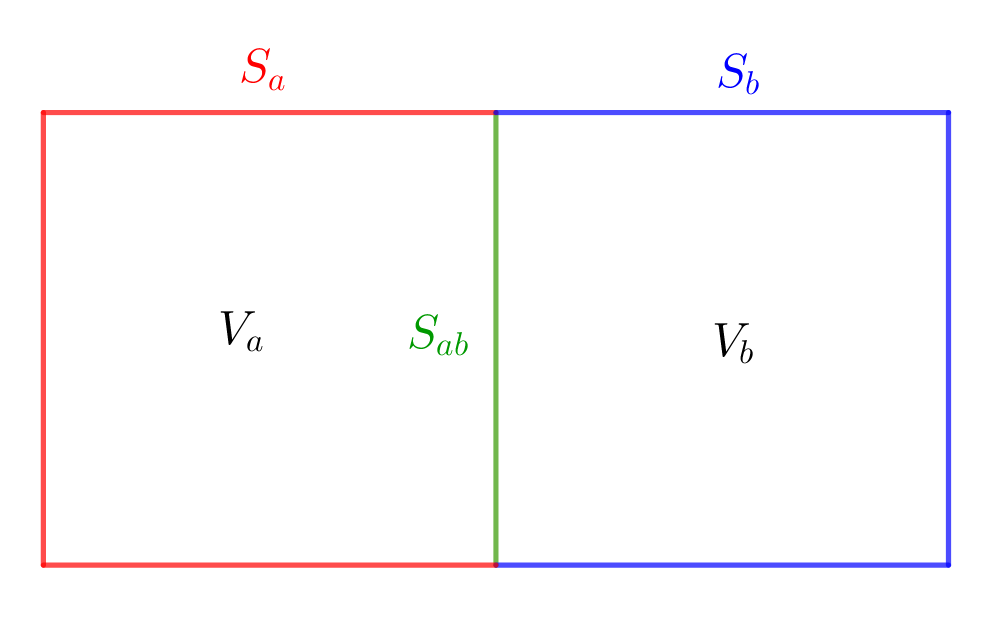
\includegraphics[width=0.7\linewidth]{fvm.png}
	\caption{A volume split into two, which splits the surface into 3 parts. Sum of integrals over the individual volumes will sum up to exactly the same as integrals over the entire volume. This is the foundation of the finite volume method.}
	\label{fig:fvm}
\end{figure}

Say we have a volume $ V $, which we split into two parts, such that $ V= V_a\cup V_b$ (see figure \ref{fig:fvm}), then the volume integral over the whole volume can be split into two:
\begin{equation*}\label{key}
	\int_{V} f(\V{x}) \ud V = \int_{V_a \cup V_b} f(\V{x}) \ud V = \int_{V_a}f(\V{x}) \ud V + \int_{V_b} f(\V{x}) \ud V.
\end{equation*}
Likewise, the surface of the volume, $ S $ is split into two such that $ S = S_a \cup S_b $, but the splitting of the volume introduces a new surface, $ S_{ab} $, such that the surface of $ V_a $ is $ \partial V_a = S_a \cup S_{ab} $ and $ \partial V_b = S_b \cup S_{ab} $. The two volume integrals sum up to the volume integral of the whole domain, likewise, the surface integrals will too:
\begin{align*}\label{key}
	\int_{\partial V_a \cup \partial V_b} \V{f}(\V{x})\D \V{n} \ud S &= \int_{\partial V_a}  + \int_{\partial V_b}  \\
	&= \int_{S_a}+\int_{S_{ab}}+\int_{S_b} - \int_{S_{ab}}\\
	&= \int_{S_a\cup S_b} = \int_S 
\end{align*}
where we have omitted the integrands and merely represented the integrals schematically. Furthermore there is a minus in front of the second integral over $ S_{ab} $ since for one control volume the surface normal points one way, and for the other it is flipped, leading to the same integral, but with a different sign.


This all means, when we split up the domain into smaller control volumes, we are guaranteed that the sum over all integrals will give the exact same solution as integrating over the whole volume in the first place. Looking at this from the view of continuity equations gives us a nice picture: The integral over the whole volume is a global conservation law, whilst the integrals over the control volumes constitutes local conservation laws.

In fact, this is all just a restating of the fact that the governing equation must be valid over the whole domain, so of course it will also, by definition, be valid over each control volume.

\section{Finite volume method for hyper elastic materials}
In this assignment we look at simulating the dynamics of hyper elastic materials using the Finite Volume Method (FVM). Where we in hand-in 5 looked at the Cauchy momentum equation with the assumption $ \ddot{x}=0 $, we will in this assignment not neglect this term, and instead employ a simple time evolution of the system to find the solution.

The governing equation is
\begin{equation}\label{key}
	\rho_0 \ddot{\V{x}} = \V{b}_0 + \grad_{0} \D \V{P}
\end{equation}
where $ \rho $ is the mass density, $ \V{b} $ is the body force density (gravity or viscosity, for example), and $ \V{P} $ is the first Piola-Kirchhoff stress tensor. A subscript of zero means the function is dependent on material, or undeformed, coordinates, meaning the last term is the divergence of the first Piola-Kirchhoff stress tensor, in material coordinates.

We impose boundary conditions on the system in the form of a nodal traction field, defined by
\begin{equation}\label{key}
	\V{P}\hat{\V{N}}=\V{t}
\end{equation}
where $ \hat{\V{N}} $ is the outward unit normal of the edge, in material coordinates, and $ \V{t} $ is a known traction field.

In our discretization we use a triangular mesh as the computational domain, with median dual vertex centred control volumes. We further assume that the deformation gradient is constant over each triangular element, meaning we get a constant $ 2\times 2 $ matrix deformation gradient for each element. Of course, this approximation is not entirely physical, since it potentially introduces discontinuities at every element border, but it simplifies calculations immensely, and in any case, it approaches the correct solution as the density of elements approaches infinity.

We further assume the mass density of the system to be constant, as we work with homogeneous materials, and only one at a time. 

\subsection{Notation, nomenclature and the control volumes}
\begin{figure}
	\centering
	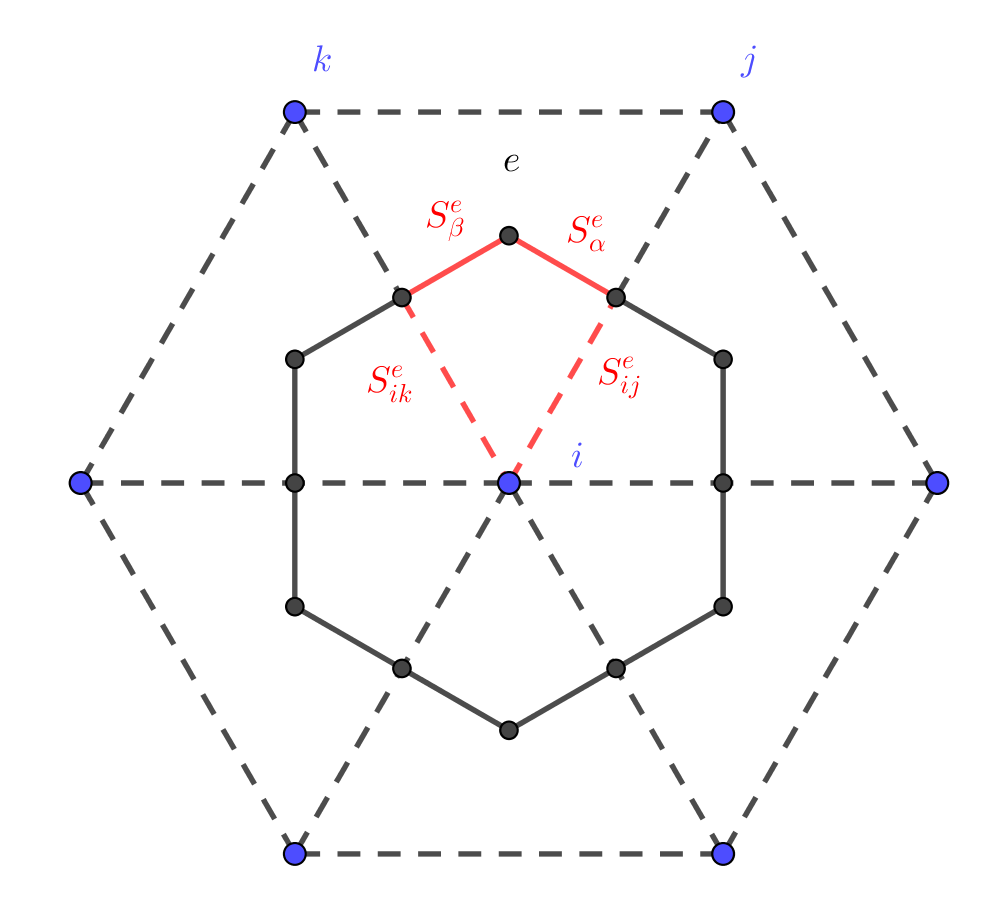
\includegraphics[width=0.7\linewidth]{CV.png}
	\caption{Sample control volume. The mesh is shown as dashed lines, whilst the control volume is shown as fully drawn lines. Also highlighted is the $ e $'th element, with vertices $ i,j,k $, along with the integration path used to simplify formula \ref{eq:integration}}
	\label{fig:CV}
\end{figure}
As with many problems, a good notation is half the battle. As mentioned before, a subscript of 0 (or capital letters for stuff other than stress tensors) denotes material coordinates, whilst lower letters and no subscript denotes spatial coordinates. We denote a element edge on the boundary of the domain as free, if there is no traction field applied to it, and non-free if there is.

The control volume we employ is slightly different than the centroid dual vertex centred control volume from last week. For each vertex $ i $, we join the incenters of each element $ e $ the vertex is a part of, to the midpoint between the vertex in question ($ i $), and the other vertices in the element $ j,k $ (see figure \textbf{ref} for a sample control volume). Using this control volume turns out to be beneficial for this governing equation with our approximations, as we shall soon see.

We denote the line segments between edge midpoints and incenters of element $ e $ as $ S^e_{\alpha} $ and $ S^e_{\beta} $, and the line segments between the $ i $'th vertex and the midpoint between the $ i $'th and $ k $'th vertex as $ S^e_{ik} $. As such, the union of these four line segments constitutes a closed curve on the domain, going from vertex $ i $ to midpoint, to incenter, to midpoint and back to vertex $ i $.


\subsection{Discretization}
Next we integrate the governing equation over the $ i $'th control volume in material coordinates, giving
\begin{equation}\label{key}
	\int_{A_i} \rho_0 \ddot{\V{x}} \ud A = \int_{A_i} \V{b}_0 \ud A + \int_{A_i} \grad_0 \D \V{P} \ud A
\end{equation}
On the left hand side we exchange the order of integration and differentiation, which we can do due to the control volume having a fixed area (in material coordinates, that is. It will deform and change in spatial coordinates). Further, with the assumption that $ \rho_0 $ is a constant we get
\begin{equation}\label{key}
	\int_{A_i} \rho_0 \ddot{\V{x}} \ud A = \rho_0 \diff[\ud]{^2}{t^2}\int_{A_i} \V{x} \ud A
\end{equation}
We then use the midpoint approximation rule and take $ \V{x} $ to be the value in the center of the control volume, ie the position of the $ i $'th vertex, giving
\begin{equation}\label{key}
	\int_{A_i} \rho_0 \ddot{\V{x}} \ud A = \rho_0 A_i \ddot{\V{x}}_i = m_i \ddot{\V{x}}_i
\end{equation}
where $ m_i $ is the ``nodal mass'', ie the mass attributed to each vertex/control volume (if we do not assume a constant density, we would just have to use the midpoint approximation for the density as well, effectively setting the density constant over each element). We give a similar treatment to the first term on the right hand side and use the midpoint rule with the value of $ \V{b}_0 $ at the $ i $'th vertex as the integrand. For the second term we just use the Gauss-divergence theorem to change the surface integral over the divergence, to a closed line integral, and then split up this line integral into piecewise continuous parts. This all gives us
\begin{equation}\label{key}
	m_i \ddot{\V{x}} = f_i^{\text{body}} + \sum_{\gamma} \int_{S^e_{\gamma}}\V{P}\hat{\V{N}} \ud S
\end{equation}
where $ f_i^{\text{body}} =A_i\V{b}_0$ is the total body force on the control volume, and $ \gamma $ runs over all edges of the control volume ($ \alpha, \beta$ for each element).

If $ S^e_{\gamma} $ is on the boundary of the domain, then it is either free or non-free. In the free case $ \V{P}\hat{\V{N}} =\V{t}=0$ and the integral vanishes. In the non-free case the integral is just $ \V{t}l^e_{\gamma}$, where $ l^e_{\gamma} $ is the length of $ S^e_{\gamma} $ ($ \V{t} $ is constant over the edge, so goes outside the integral, and the integral of 1 is just the edge length).

With this we can split up the piecewise integral further into boundary edges and inner edges. The integral over inner edges can be calculated without even using the $ \alpha, \beta $ edges if we utilize the closed contour mentioned before. Since we assume that the tensor $ \V{P} $ is constant over each element, the integral of a closed contour on the element is zero (like that of a gradient or any field with a vanishing curl):
\begin{equation}\label{eq:integration}
	\oint_S \V{P}^e\hat{\V{N}} \ud S = 0
\end{equation}
Now we let $ S = S^e_{ji} \cup S^e_{ik} \cup S^e_{\alpha} \cup S^e_{\beta} $, giving
\begin{equation}\label{key}
	\V{f}^e_i = \int_{S^e_{\alpha} \cup S^e_{\beta}} \V{P}^e\hat{\V{N}} \ud S = -\int_{S^e_{ji} \cup S^e_{ik}} \V{P}^e\hat{\V{N}} \ud S
\end{equation}
Next we note that $ \V{P}^e $ is constant by assumption (the deformation gradient is constant, giving a constant stress tensor), and $ \hat{\V{N}} $ is constant along each straight edge, so $ \V{f}^e_i $ is given by
\begin{equation}\label{key}
\V{f}^e_i = -\frac{1}{2} \V{P}^e \hat{\V{N}}^e_{ji}l_{ji} - \frac{1}{2} \V{P}^e\hat{\V{N}}^e_{ik}l_{ik}
\end{equation}
with $ l_{ik} = |\V{x}_k - \V{x}_i|$. Computations can be saved by noting that $ \hat{\V{N}}^e_{ji} l_{ji} $ is just the vector $ \V{x}_i-\V{x}_j $ rotated by 90 degrees, such that it points outward of the element (counter clockwise). Likewise with $ \hat{\V{N}}^e_{ik} l_{ik} $ being $ \V{x}_k -\V{x}_i$ rotated 90 degrees counter clockwise (note the order of the indices, first index is starting point, last index is ending point).

Putting all of this together, we get the final equation of motion for the $ i $'th vertex:
\begin{equation}\label{key}
	m_i \ddot{\V{x}}_i = \V{f}_i^{\text{body}} + \V{f}_i^t +\V{f}^E_i, \quad \V{f}^t_i = \sum_{\gamma}   \V{t}l^e_{\gamma}, \quad \V{f}^E_i = \sum_e \V{f}^e_i
\end{equation}
where $ \V{f}^t_i $ is the total traction force, made up of contributions from each non-free boundary edge, and $ \V{f}^E_i $ is the total elastic force, made up of contributions from each element of the $ i $'th control volume (ie, all elements the $ i $'th vertex is a part of).

Now, this is all well and good, but we still have not calculated the first Piola-Kirchhoff stress tensor $ \V{P} $. The tensor is given by $ \V{P} = \V{F}\V{S} $, with $ \V{F} $ being the deformation gradient and $ \V{S} $ being the second Piola-Kirchhoff sress tensor. This is given by
\begin{equation}\label{key}
	\V{S} = \lambda \tr (\V{E}) \V{I} + 2 \mu \V{E}, \quad \V{E} = \frac{1}{2} (\V{F}^T \V{F} - \V{I})
\end{equation}
where $ \V{E} $ is the Green strain tensor and $ \lambda, \mu $ are the first and second Lame coefficient, which can be calculated from the Young Modulus $ E $ and Poisson Ratio $ \nu $ by
\begin{equation}\label{key}
	\lambda = \frac{E\nu}{(1+\nu)(1-2\nu)}, \quad \mu = \frac{E}{2(1+\mu)}.
\end{equation}
The can has been kicked down the road long enough now, we just need the deformation gradient for each element, then we are golden. The deformation gradient is what takes the material coordinates to the spatial coordinates, and since we assume the deformation gradient to be constant, we can find it quite simply. For the $ e $'th element we define $ \V{g}_{ij}^e =\V{x}_j - \V{X}_i,\V{G}_{ij}^e =\V{X}_j - \V{X}_i $. These vectors are related by the deformation gradient with
\begin{equation}\label{key}
	\V{g}_{ij}^e = \V{F}^e \V{G}^e_{ij}
\end{equation}
So if we let $ \V{D}^e = [\V{g}^e_{ij}\ \V{g}^e_{ik}], \V{D}^e_0 =  [\V{G}^e_{ij}\ \V{G}^e_{ik}]$ we get
\begin{equation}\label{key}
	\V{D}^e = \V{F}^e \V{D}^e_0, \quad \V{F}^e = \V{D}^e (\V{D}^e_0)\inverse
\end{equation}
This has the advantage that the matrix inverse is only dependent on the material coordinates, which by definition are constant - so these matrices can be precomputed!

With all of this done we are now in a position where we can calculate the total forces on each vertex for a given time step. All we then need is to update the positions of the vertices to evolve the system in time. For this we employ a semi-implicit first order finite difference approximation.

We let $ \V{v}_i = \dot{\V{x}}_i $, giving us a pair of coupled first order ODEs by
\begin{align}\label{key}
	\dot{\V{v}}_i &= \frac{1}{m_i} \V{f}_i^{\text{total}} = \frac{1}{m_i}(\V{f}^{\text{body}}_i + \V{f}^t_i + \V{f}^E_i), \\
	\dot{\V{x}}_i &= \V{v}_i.
\end{align}
With the FDM approximation giving
\begin{align}\label{key}
	\V{v}_i^{t+\Delta t} &= \V{v}_i^{t} + \frac{\Delta t}{m_i} \V{f}^{\text{total}}_i, \\
	\V{x}_i^{t+\Delta t} &= \V{x}_i^t +\Delta t \V{v}_i^{t+\Delta t}.
\end{align}
Note that we use an explicit updating scheme for the velocity, but an implicit updating scheme for the position, hence the name ``semi-implicit time integration''.

To evolve the system in time by one time step, we need to calculate the total forces, which entails computing all deformation gradients, to calculate all element stress tensors. With the total force on the $ i $'th vertex calculated, we can then update the position and velocity of this vertex.

Note that this that all coupling between elements occur in computing the total forces (the elastic forces, actually), and we do not need to perform any matrix assembly and solving, in contrast to all the other weeks assignments (except for semi-lagrangian impicit time integration).

\subsection{Parameters and energies}
For all of this weeks experiments we will be using a Young Modulus $ E =1000 $ Pa, Poisson ratio $ \nu=0.3 $, mass density $ \rho_0=10  $kg/m$ ^2 $. The Lame parameters are calculated from the equations
\begin{equation}\label{key}
	\lambda = \frac{E\nu}{(1+\nu)(1-2\nu)}, \quad \mu=\frac{E}{2(1+\nu)}
\end{equation}
These values are pitiful. Especially the Young Modulus. Steel, for example, has a Young Modulus of around 100 GPa, a difference of 7 orders of magnitude! So we are essentially working with solidified pudding.

In the experiments we will also calculate the energy present in the system. We will calculate 3 different energy contributions: kinetic, gravitational potential and strain energy. The first two are given by
\begin{equation}\label{key}
	E_{\text{kin}} = \sum_{i} \frac{1}{2} m_i v_i^2, \quad E_{\text{pot}} = \sum_{i} m_i g (y_i-y_0)
\end{equation}
where the sums are over all vertices, and $ y_0 $ is some arbitrarily defined 0-point for the gravitational energy, taken to be 0 for all experiments. The strain energy is found by integrating the strain energy density function $ \psi $ over the whole material. The function is given by
\begin{equation}\label{key}
\psi = \frac{1}{2} \lambda \tr (\V{E})^2 + \mu \tr (\V{E}^2)
\end{equation}
but since $ \V{E} $ is constant over each element, we can replace the integral with a sum over elements:
\begin{equation}\label{key}
	E_{\text{str}} = \int_V \psi \ud V = \sum_{e} \psi^e A^e_0
\end{equation}
where $ A^e_0 $ is the area of the $ e $'th element, in material coordinates.


\section{Experiments}
\subsection{An oscillating triangle}
\begin{figure}
	\centering
	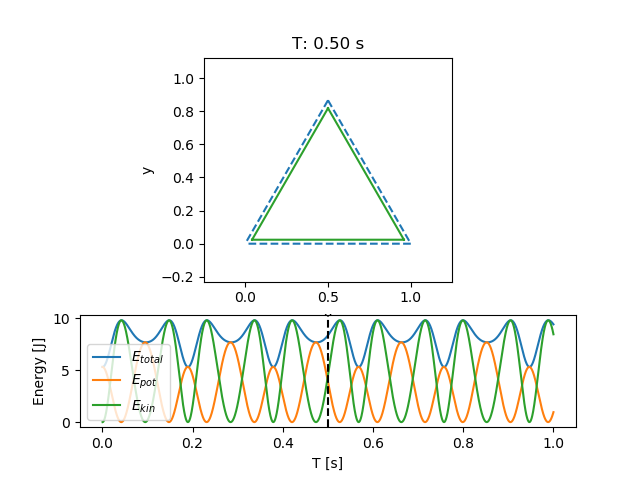
\includegraphics[width=\linewidth]{triangle.png}
	\caption{Snapshot of the oscillating triangle simulation. The material mesh are plotted with dashed lines, while the spatial mesh is plotted with solid lines. Also shown is the energy of the system, as a function of time. While the energy is not constant, there does not seem to be any dissipation of energy either.}
	\label{fig:triangle_sim}
\end{figure}
For the first experiment, we do perhaps the simplest of experiments. We create a computational mesh consisting of 3 vertices, arranged to form an equilateral triangle, with its centre coinciding with the origin. This will be the material coordinates. Next we scale the triangle by $ a>1 $ uniformly. The elastic forces will then tend to contract the triangle towards its relaxed state, but it will overshoot due to the gain in velocity, compressing the triangle, and introducing a restoring force in the opposite direction, forming a harmonic oscillator.

We set the traction and any body forces to zero, and use this as an experiment to verify the elastic forces. We also expect the total energy, the sum of strain and kinetic energies, to be constant.

Letting the simulation run and plotting it gives the result seen in figure \ref{fig:triangle_sim}, with the full video available at \textbf{LINK}. As seen, the potential energy oscillates but with differing amplitudes for compression and expansion, so there is either an error in calculating the strain energy, or some other energy contribution we are forgetting. The gravitational potential energy is constant, since the centre of mass is at the geometric centre, which does not move, so this is not the cause for the mismatch (it does not make sense to calculate it either. By not including it we essentially set $ g=0 $, which would lead to no gravitational potential energy either). Further, calculating the strain energy analytically for the system with a deformation gradient of $ aI $ gives
\begin{equation}\label{key}
	E_{\text{str}} = \frac{\sqrt{3}}{8} (a^2-1) (\lambda+\mu)
\end{equation}
Calculating this expression explicitly in the code and comparing it to the starting strain value calculated by the simulation yields an expression which is accurate down to a couple of machine epsilon.

So it looks like there is some contribution which we are forgetting.

However, the values at the peaks of the different energies (kinetic, strain and total) do not decay - there seems to be no dissipation of energy, which is like we expect. This is also the case when running the simulation for 10 times as long. Though the energy graph becomes a blurry mess, so we decided against plotting this.



\subsection{Bending the bar}
\begin{figure}
	\centering
	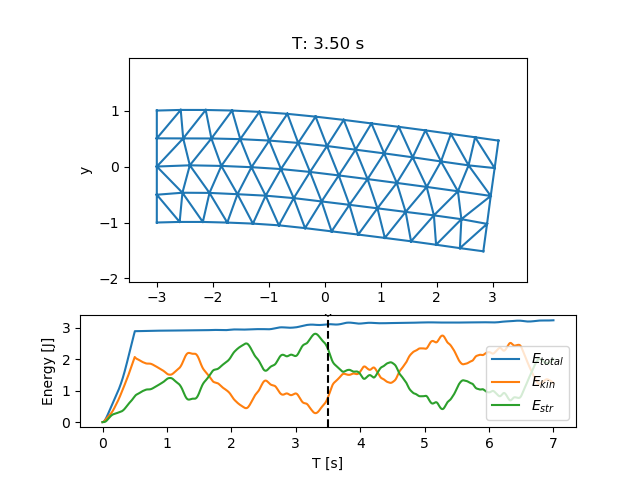
\includegraphics[width=\linewidth]{bar.png}
	\caption{Snapshot of the second experiment. Notice that the energy increases rapidly at the start of the simulation, as the traction performs work on the system. The total energy does not settle to a constant after the traction is released at $ T=0.5$s as one would expect. We do see a trade-off in the strain and kinetic energy as the bar bends back and forth, though.}
	\label{fig:bar}
\end{figure}
For the second experiment we repeat the bending of the bar from the experiments of the finite element method in week 5. We use the provided mesh from that week, attach the left end to a ``wall'' and apply a constant traction to the right end for some time period ($ T = 0.5  $ s), whereupon we set the traction to 0. This will act as an ``initial displacement'' like for the oscillating triangle. Unlike the triangle though, we have an added ``initial'' velocity, and some build-up of errors. We also neglect any body forces such as gravity, meaning the only forces are the traction and elastic forces.

In attaching the left end to the wall we essentially negate all forces on these nodes (The wall exerts an equal force on the bar, so to speak), such that these nodes never move. In practice this means we just set the velocity for these nodes to 0, and never update them.

As the bar is released we expect it to behave like a harmonic oscillator with an initial displacement and initial velocity different from 0. The result is seen in figure \ref{fig:bar}, with the full simulation available at \textbf{LINK}.

At first, the traction performs work on the bar, which is why we see the total energy increase for the first 0.5 seconds. Then a peculiar thing happens: The bar starts to wobble, and we se ``shock-waves'' in the material, as the discontinuity in acceleration propagates back and forth through the system - hitting the wall and being reflected back (with a negative amplitude), which is precisely what we see if we have a rope attached to a wall, and send a transverse wave down the length of it!

This is also what gives the ``wobbles'' in the trade-off between kinetic and strain energy. An observation leading to slight disconcert is the fact that the total energy in the system continues to increase as the 


\subsection{A bouncing ball}
We can also use this method to simulate a bouncing ball. To do this we need a circular mesh, gravity and a procedure for handling collision with the floor.

Applying gravity is easy: we just apply body force density of $ \rho_0\V{g}=\rho_0[0, -g]^T $. Next the procedure for the floor. When a ball hits a floor, the upwards momentum of the ball will die out (if the floor is perfectly rigid), causing the ball to compress. This introduces a deformation gradient and elastic forces in the vertical direction, counteracting the gravitational forces. At some point, these forces are greater than the gravitational pull, causing the ball to accelerate and jump back up.

So whenever a vertex is at or under the floor (defined as the region below some $ y=y_0 $, taken to be $ 0 $ for simplicity), we push it back up to the floor and set its vertical component of velocity to 0. This then induces the deformation, hopefully creating the scenario described above.

We should see conservation of energy in this case: At first, the energy is entirely stored as potential energy. As the ball falls however, the potential energy is converted into kinetic energy, until the ball reaches the floor, at which point the ball bounces, turning the downward momentum to upward momentum. The ball then deccelerates converting the kinetic energy back into potential energy.

Of course, perfect energy conservation depends on whether or not the collision with the floor is elastic or inelastic. I have my doubts that it will be completely elastic due to the fact that we set the vertical velocity component to 0, killing off some of the systems kinetic energy. The hope is that this loss will be stored as ``potential'' energy in the elasticity of the ball. So hopefully we see a nice constant total energy, with potential and kinetic energy trading off each other, back and forth forever.

\end{document}
